\documentclass[a4paper,12pt,twoside]{ThesisStyle}
\usepackage[utf8]{inputenc}
\usepackage{thesis-style}
\usepackage[english]{babel}

\begin{document}

\frontmatter

\pagenumbering{gobble}

\thispagestyle{empty}
\begin{table}[htb]
  \centering
  \begin{Large}
    \resizebox{\textwidth}{!}{\begin{tabular}{ | l |}
        \hline
        \\
        
\includegraphics[scale=0.9]{img/logo_eps.png}    \\[0.7cm]
        \centerline{Treball Final de Màster}                 \\[1cm]
        \hline
        \\
        Estudi: Màster en Ciència de Dades                   \\[0.7cm]
        \hline
        \\
        Títol: Ajustament d'un model generatiu de llenguatge \\
        per a la creació de xatbots personalitzats per       \\
        administracions públiques                            \\[0.7cm]
        \hline
        \\
        Document: Memòria                                    \\[0.7cm]
        \hline
        \\
        Alumne: Martí Mas Fullana                            \\[0.7cm]
        \hline
        \\
        Tutor: Josep Suy Franch                              \\
        Tutor: Miquel Tarragona Margarit                     \\[0.7cm]
        Departament: Departament d'Informàtica, Matemàtica   \\
        Aplicada i Estadística                               \\
        Àrea: Intel·ligència Artificial                      \\[0.7cm]
        \hline
        \\
        Convocatòria (mes/any): Setembre 2024                \\[0.7cm]
        \hline
      \end{tabular}}
  \end{Large}
\end{table}

\newpage
\hypersetup{pageanchor=false}
\begin{titlepage}

  % Upper part of the page
  
\includegraphics[scale=0.9]{img/logo_eps.png} \\[1cm]
  \begin{center}
    \textsc{\Large Master's Thesis} \\[1cm]

    % Title
    \begin{spacing}{2}
      \HRule \\
      \textbf{\Huge Tuning a Generative Language Model for the Creation of Customized Chatbots for Public Administrations} \\
      \HRule \\[0.5cm]
    \end{spacing}

    % Author and supervisor and other data
    {
    \large
    \emph{Author:} \\
    Martí \textsc{Mas Fullana} \\[1cm]
    Setembre 2024 \\[1cm]
    Master's in Data Science \\[1cm]
    \emph{Supervisor:} \\
    Josep \textsc{Suy Franch} \\
    }

  \end{center}
\end{titlepage}
\hypersetup{pageanchor=true}

\titlepage

%\dominitoc


\pagenumbering{roman}

\chapter*{Summary}
\label{cap:summary}

% This document presents the architecture and methodology for developing an advanced chatbot system that uses GPT (Generative Pre-trained Transformer) technology and RAG (Retrieval Augmented Generation) to provide assistance with social rights and benefits in Catalonia. The system aims to improve the accuracy and relevance of responses generated by chatbots by combining the strengths of information retrieval from a database with the generative capacity of language models. The system consists of a frontend interface implemented in Angular, a backend that manages the conversation flow and communicates with Azure services such as Speech-to-Text and a PostgreSQL database, and a Vector Search API that handles information retrieval and response generation. The methodology involves data collection and preparation, implementation of the RAG system, user interface design, and evaluation and validation of the system. The objectives of the project include selecting an appropriate GPT model, integrating RAG technology, facilitating user-chatbot interaction, ensuring accessibility, and evaluating and validating the system. The document also provides background information on dialogue systems, GPT, and RAG, as well as the objectives and architecture of the project.

This document presents the design and implementation of a customized chatbot system utilizing GPT (Generative Pre-trained Transformer) and RAG (Retrieval Augmented Generation) technologies to enhance public administration services in Catalonia, specifically for social rights and benefits. The system integrates a frontend interface in Angular with a backend that manages conversational flow and connects with Azure services such as Speech-to-Text and a PostgreSQL database. The backend also employs a Vector Search API for information retrieval and response generation. Key components include data collection and preparation from public websites, implementation of the RAG framework for precise information retrieval, and the development of a user-friendly, multilingual interface with accessibility features. The system's architecture is modular, enabling adaptability for future applications, and is validated through user testing and performance analysis, aiming to improve accuracy, relevance, and user satisfaction while minimizing operational costs.

\chapter*{Acknowledgements}
\label{cap:acknowledgements}

I would like to express my gratitude to my tutor Josep Suy Franch for his guidance and support throughout the development of this project. I would also like to thank Benjamí Fuertes, Sergi Martinez and Joan Oller for their hard work and dedication to the project, and for their patience answering my questions, as well as thank DXC Technology for providing me with this opportunity. I thank my family and friends for their encouragement and understanding during this time.
Finally, I would like to thank my fiancée for her unwavering love and support.


\tableofcontents

\listoffigures

\listoftables

\mainmatter

\chapter{Introduction}
\label{cap:intro}

We present a chatbot system that uses GPT (Generative Pre-trained Transformer) technology and RAG (Retrieval Augmented Generation) to provide assistance with social rights and benefits in Catalonia. Our client is the department of social rights of the Generalitat de Catalunya (\textit{Departament de Drets Socials} or DSO). This thesis has been developed in collaboration with \bolditalic{DXC Technology}.

\section{About DXC Technology}
\label{sec:dxc}

\begin{figure}[htb]
  \centering
  
\includegraphics[width=0.5\textwidth]{img/DXC_Technology_Logo.png}
  \caption{DXC Technology Logo}
  \label{fig:dxc_logo}
\end{figure}

DXC Technology is a global IT services company that provides a wide range of services to clients in various industries. It has a strong presence in the public sector, providing IT solutions to government agencies and public administrations. The company has a long history of working with public sector clients to develop innovative solutions that improve service delivery and enhance citizen engagement.

DXC Technology is a multinational corporation employing over 130,000 people in over 70 countries, headquartered in Tysons, Virginia, USA. In Spain it has offices in Madrid, Barcelona, Valencia, Bilbao, Sevilla, Madrid and Girona.

\section{Key Terms and Definitions}
\label{sec:terms}

\begin{itemize}
  \item \textbf{DSO:} \textit{Departament de Drets Socials}, the Department of Social Rights of the Generalitat de Catalunya. This department is responsible for managing social benefits and services in Catalonia.
  \item \textbf{SNOMED:} A SNOMED, short for Systematized Nomenclature of Medicine, is a code that represents a medical concept. For example, the SNOMED code for ``diabetes'' is 73211009.
  
  For reasons not relevant to this project, the Department of Social Rights uses SNOMEDs to represent a user's situation. These SNOMEDs are used to determine which social benefits a user might be eligible for. For example, they have a SNOMED for ``Sexist Violence at Home''. As we will see in chapter \ref{cap:architecture}, we have a component called \textit{IA Social} that can infer which SNOMEDs might apply to a user based on the conversation.
  \item \textbf{Products:} These are the actual social benefits that the user might be eligible for. These might entail things like monetary aid, legal assistance, or other forms of support. The products are determined by the SNOMEDs that apply to the user. The Department of Social Rights provides us with an API called ``kSocial'' (``k'' is for ``Katalog'') that we can use to query which products are available for a given set of SNOMEDs.
  \item \textbf{Embedding:} An embedding is a vector representation of a piece of data. Embeddings capture high-level semantic information about the data they represent, and are used in machine learning models to perform tasks such as information retrieval and classification. Embeddings are ususally high-dimensional, with hundreds or thousands of dimensions.
  
  Embeddings are computed by encoder neural networks, and can be used either to later decode them for a specific task (like generating text, as in the case of GPT models) when paired with appropriate decoder neural networks; or directly used for tasks like information retrieval.
  
  In this document, embeddings will refer to Float32 vectors of 3072 dimensions, which store the semantic information of text chunks; except in the case of the embeddings generated by the Hotword Detector (see section \ref{subsec:hotword_detection}), which are 2048-dimensional vectors storing the semantic respresentations of 1.5-seconds-long Mel spectrograms. In all cases these vectors will have a modulus of 1, which simplify the computation of cosine similarity to merely the dot product of the vectors, for compute efficieny.
\item \textbf{Zero-shot Learning:} Zero-shot learning refers to the model's ability to handle a task without having been directly trained on any examples of that specific task. In other words, the model generates responses or performs actions based purely on its general understanding of language, knowledge, and context gained from pre-training on vast and diverse text corpora.
\item \textbf{Few-shot learning:} Few-shot learning is a technique where the model is given only a few examples (or "shots") of a particular task during inference to understand how to perform that task. Unlike zero-shot learning, where no examples are provided, few-shot learning leverages a small number of examples provided in the prompt to guide the model’s behavior.
\end{itemize}

\chapter{Background}
\label{cap:background}

\section{Introduction to Dialogue Systems}
\label{sec:chat}

Dialogue systems, also known as chatbots, have experienced a significant step-change in the last few years. Initially these systems were based on predefined rules and decision trees \cite{Weizenbaum1966ELIZA, AbuShawar2015ALICE}, limiting their capacity for understanding and answering user queries in a natural and flexible manner. These rudimentary systems, commonly referenced as rule-based chatbots, might have been enough for simple tasks, but could not have managed the full complexity and variability of natural language.

\section{Towards Language Models}
\label{sec:language}

As the first machine learning-based language models appeared, such as the Sequence-to-Sequence (Seq2Seq) model \cite{Sutskever2014SequenceSequenceLearningNeural}, and more recently the transformer-based models such as GPT (Generative Pre-trained Transformer) \cite{Vaswani2023AttentionNeed, Radford2018GPT1}, the capacity of chatbots to understand and generate natural language has improved significantly. These models are trained on large datasets of text, learning the complex patterns and structures of language, and are able to generate text that is coherent and contextually relevant.

\section{GPT and its Contribution}
\label{sec:gpt}

The GPT model \cite{Radford2018GPT1}, developed by OpenAI, has been one of the most notable advances in this field. GPT uses the transformer architecture \cite{Vaswani2023AttentionNeed}, which is a type of neural network that is particularly well-suited for processing sequences of data, such as text. Its capacity for generating coherent and contextually relevant responses has been leveraged in a wide range of applications, from virtual assistance to automated content generation.

In the following subsections we will go over the evolution of the GPT model, from GPT-1 to GPT-4.

\subsection{GPT-1}
\label{subsec:gpt-1}

GPT-1 \cite{Radford2018GPT1}, introduced by OpenAI in 2018, marked the beginning of the Transformer-based language models. It used the Transformer architecture, a neural network model that significantly improved over earlier models like recurrent neural networks (RNNs) and Long Short-Term Memory (LSTM) networks. The key innovation in GPT-1 was its ability to generate coherent text by predicting the next word in a sequence, trained on a vast dataset of books and articles. With 117 million parameters, GPT-1 demonstrated that a generative model, pre-trained on a large corpus of text data, could be fine-tuned on specific tasks to achieve good performance across a variety of NLP applications. Although it was relatively small in terms of model size and capacity, GPT-1 established the foundational approach of using unsupervised pre-training followed by supervised fine-tuning.

\subsection{GPT-2}
\label{subsec:gpt-2}

Building on the success of GPT-1, GPT-2 \cite{Radford2019GPT2} was released in 2019 and significantly increased in size, with versions ranging up to 1.5 billion parameters. GPT-2 demonstrated substantial improvements in language understanding, coherence, and the ability to generate more human-like text. It was trained on a much larger and more diverse dataset, which included a wide range of web pages, allowing it to handle more complex language tasks. GPT-2 could perform zero-shot learning, meaning it could complete tasks without specific training on those tasks, just by leveraging the general knowledge it gained during its pre-training phase. This version showcased the model's capacity to handle a wide range of tasks, from text completion and summarization to translation and question answering, making it a significant milestone in AI research. It was the first model to demonstrate the potential for large-scale language models to generate high-quality text across a variety of domains, and the potential of simply scaling up model size to improve performance.

\subsection{GPT-3}
\label{subsec:gpt-3}

Released in 2020, GPT-3 \cite{Brown2020GPT3} took another leap in scale and capability with 175 billion parameters, making it one of the largest language models at the time. GPT-3's vast size allowed it to exhibit unprecedented levels of language understanding and generation. It could produce highly coherent and contextually relevant text across diverse topics, maintain longer and more complex conversations, and even exhibit rudimentary reasoning skills. GPT-3 was capable of few-shot and zero-shot learning, further extending its versatility. However, GPT-3 was also computationally expensive and required significant resources for both training and inference, which limited its accessibility.

\subsection{Reinforcement Learning from Human Feedback (RLHF)}
\label{subsec:rlhf}

\cite{Ouyang2022RLHF} introduced Reinforcement Learning from Human Feedback (RLHF), which marked a significant step forward in the development of GPT models. RLHF is a technique where the model is fine-tuned using feedback from human evaluators who assess the quality of the model's outputs. This method involves the following steps:


\begin{itemize}
  \item \textbf{Pre-training:} The model is initially pre-trained on a large text corpus using unsupervised learning, just like previous versions.
  \item \textbf{Human Feedback Collection:} Human evaluators review the model's responses to various prompts and rank them based on quality, coherence, relevance, and other criteria.
  \item \textbf{Reward Model Training:} A separate reward model is trained on these rankings to predict the human evaluators' preferences.
  \item \textbf{Fine-tuning:} The GPT model is further fine-tuned using a reinforcement learning algorithm, such as Proximal Policy Optimization (PPO) \cite{Schulman2017ProximalPolicyOptimizationAlgorithms}, where the reward model guides the optimization to produce outputs more aligned with human preferences.
\end{itemize}

By incorporating RLHF, GPT models learn not only from the data they are trained on but also from direct human feedback, allowing them to better align with human values, reduce harmful or biased outputs, and improve overall user satisfaction.

\subsection{GPT-3.5 Turbo}
\label{subsec:gpt-3.5-turbo}

To optimize GPT-3's capabilities for commercial use, OpenAI released GPT-3.5 Turbo, a more efficient variant of GPT-3.5, designed to offer improved performance while reducing computational costs. GPT-3.5 Turbo maintained much of the language understanding and generation quality of GPT-3 but was optimized for lower latency and more cost-effective deployment, making it suitable for a wider range of applications, including real-time interactive systems like chatbots. It also incorporated the improvements from RLHF to enhance the model's ability to generate high-quality text, follow instructions and align with human preferences.

\subsection{GPT-4o and GPT-4o Mini}
\label{subsec:gpt-4o}

GPT-4o \cite{gpt4o} represents the latest iteration in OpenAI's series of language models, featuring further advancements in both scale and architecture. GPT-4o builds upon the lessons learned from earlier models and introduces several optimizations to enhance performance and efficiency. The ``o'' in GPT-4o stands for ``omni'', reflecting the model's focus on multimodal capabilities (the ability to process and generate text, images, voice and video) and its versatility across a wide range of tasks and domains. GPT-4o is designed to deliver state-of-the-art performance in language understanding and generation, with a focus on accuracy, coherence, and contextuality. From \cite{gpt4o}: ``GPT-4o [...] is a step towards much more natural human-computer interaction —it accepts as input any combination of text, audio, image, and video and generates any combination of text, audio, and image outputs.'' and ``It can respond to audio inputs in as little as 232 milliseconds, with an average of 320 milliseconds [...]''.

Alongside GPT-4o, OpenAI also developed the GPT-4o Mini, a smaller, more efficient version designed to deliver a substantial portion of the performance of the full GPT-4o model at a fraction of the computational cost. This model provides an excellent balance between performance and efficiency, making it ideal for deployment in production environments where cost-effective, high-quality language understanding and generation are needed.

At the time of writing there are no published papers on GPT-4o or GPT-4o Mini, and there is very little technical information available. However, based on the information provided by OpenAI, rumors and leaks \cite{betts_moe_2023}, we can infer that GPT-4o uses the latest developments in Mixture of Experts (MoE) \cite{huggingface_moe_2023}, amongst other techniques, to improve performance and efficiency.

\section{Retrieval Augmented Generation (RAG)}
\label{sec:rag}

One of the most recent advances in the integration of language models has been the use of retrieval augmented generation (RAG) \cite{Lewis2021RetrievalAugmentedGeneration}. RAG combines the strengths of information retrieval from databases with the generative capacity of language models. In this context, when a user query is received, the system first retrieves relevant information from a database, and then the language model generates a coherent and precise response based on this information. This approach has been shown to improve the accuracy and relevance of the responses generated by chatbots \cite{Lewis2021RetrievalAugmentedGeneration}.

\section{Applications and Benefits of RAG-based Chatbots}
\label{sec:applications}

RAG-based chatbots offer a variety of benefits compared with more traditional systems. They are able to generate responses that are more coherent and contextually relevant. In this way users are both less frustrated and more satisfied, thus improving user experience. These systems also allow the chatbots to have access to newer, more up to date information than the data the model was originally trained on, as the data provided to the information retrieval component can be updated by simply adding new entries to the database. This makes the chatbot more adaptable and flexible, and allows it to provide more accurate and relevant information to users, reducing the necessity of performing full or partial retraining of the model, which can be prohibitively expensive.

\chapter{Objectives}
\label{cap:objectives}

The main goal of this project is to develop an advanced chatbot system that uses GPT (Generative Pre-trained Transformer) technology and RAG (Retrieval Augmented Generation) to provide responses to user queries based off of the content of a database. This general goal can be broken down into the following specific objectives:

\begin{enumerate}
  \item \textbf{Pick an appropriate GPT Model}
        \begin{itemize}
          \item Choose a GPT model that is well-suited for the task of generating responses to user queries based on the content of a database.
        \end{itemize}
  \item \textbf{Integrate RAG Technology}
        \begin{itemize}
          \item \textbf{Information Retrieval:} Develop and implement a system for retrieving relevant information from a database based on user queries.
          \item \textbf{Combine Retrieval and Generation:} Integrate the information retrieval system with the GPT model to generate coherent and contextually relevant responses to user queries.
        \end{itemize}
  \item \textbf{Facilitate User-Chatbot Interaction}
        \begin{itemize}
          \item \textbf{UI Design} Develop a user interface that allows users to interact with the chatbot in a natural and intuitive way.
          \item \textbf{UX Design} Ensure that the user experience is smooth and seamless, and that users are able to easily access the information they need.
        \end{itemize}
  \item \textbf{Accessibility}
        \begin{itemize}
          \item \textbf{Multilingual Support} Implement support for multiple languages to make the chatbot accessible to a wider range of users.
          \item \textbf{Accessibility Features} The system must be designed to be accessible to users with visual or motor impairments. As such, it should support voice input. The voice input feature must support activation through a voice command.
        \end{itemize}
  \item \textbf{Evaluate and Validate the System}
        \begin{itemize}
          \item \textbf{User Testing} Conduct user testing to assess the usability and effectiveness of the chatbot system.
          \item \textbf{Results Analysis} Analyze the results of the different tests to identify areas for improvement and optimization.
        \end{itemize}
\end{enumerate}

\chapter{Methodology}
\label{cap:methodology}

\section{SCRUM Methodology}

The development of this project was carried out using the SCRUM methodology, an agile framework that facilitates iterative and incremental progress. SCRUM was chosen for its flexibility and ability to adapt to changes, making it well-suited for the dynamic nature of software development projects that are partially research-based.

\subsection{SCRUM Roles}

In our SCRUM process, the following roles were defined:
\begin{itemize}
    \item \textbf{Product Owner:} The Product Owner was responsible for defining the vision of the project and prioritizing the backlog. They ensured that the development team focused on delivering features that provided the most value to the stakeholders.
    \item \textbf{SCRUM Master:} The SCRUM Master facilitated the process by removing impediments, ensuring that the team adhered to SCRUM practices, and fostering a collaborative environment. They acted as a bridge between the development team and the Product Owner.
    \item \textbf{Development Team:} Composed of multidisciplinary members, the Development Team was responsible for delivering the product increments. Each team member contributed to different aspects of the project, including frontend and backend development, database management, and model integration.
\end{itemize}

\subsection{Sprint Planning}

The project was divided into multiple sprints, each lasting two weeks. During Sprint Planning meetings, the Development Team collaborated with the Product Owner to select user stories from the product backlog, which were then broken down into smaller, manageable tasks. Each task was assigned a story point value based on its complexity, and the team committed to completing a set of tasks during the sprint.

\subsection{Daily Stand-ups}

Daily stand-up meetings were held to maintain transparency and ensure smooth communication within the team. During these brief meetings, each team member shared what they accomplished the previous day, what they planned to work on that day, and any blockers or impediments they faced. This practice helped identify issues early and allowed for quick adjustments to the plan if necessary.

\subsection{Sprint Review and Retrospective}

At the end of each sprint, a Sprint Review meeting was conducted, where the team demonstrated the product increment to the Product Owner and stakeholders. Feedback was gathered, and any necessary adjustments were noted for future sprints.

Following the Sprint Review, the team conducted a Sprint Retrospective. This meeting focused on evaluating the sprint process, identifying what went well, what could be improved, and creating actionable plans for enhancing future sprints. The Retrospective was critical in fostering continuous improvement within the team.

\subsection{Backlog Refinement}

Backlog refinement sessions were held regularly to ensure that the product backlog remained up-to-date and aligned with the project goals. The team reviewed and re-prioritized user stories, added details to upcoming tasks, and estimated their complexity. This process helped the team prepare for future sprints and maintain a clear understanding of the project trajectory.

\subsection{Benefits of Using SCRUM}

The application of SCRUM in this project provided several benefits:
\begin{itemize}
    \item \textbf{Adaptability:} The iterative nature of SCRUM allowed the team to quickly adapt to changes in requirements or priorities, ensuring that the project stayed aligned with stakeholder expectations.
    \item \textbf{Collaboration:} Regular communication and feedback loops fostered a collaborative environment, enabling the team to work more effectively and efficiently.
    \item \textbf{Transparency:} The use of daily stand-ups and sprint reviews increased transparency, allowing stakeholders to stay informed of progress and providing opportunities for early feedback.
    \item \textbf{Continuous Improvement:} The focus on retrospectives ensured that the team continually refined their processes, leading to better performance and higher-quality deliverables.
\end{itemize}

By adhering to SCRUM principles and practices, the team was able to deliver a high-quality chatbot system that met the needs of the Department of Social Rights of the Generalitat de Catalunya in a timely and efficient manner.

\section{Data Collection and Preparation}
\label{sec:data}

\begin{itemize}
  \item \textbf{Data Collection:} We are given by the stakeholders a set of websites documenting the laws related to social rights in Catalonia and also documenting available social benefits. These websites contain a variety of information, including the text of the laws and the social benefits, what conditions are necessary to access them, and how to apply for them.
  \item \textbf{Data Preparation:} We will extract the text from the websites using web scraping and convert them into a format that can be used by the information retrieval system. This will involve cleaning the text and removing any extraneous characters. This will be done using custom web scraping scripts.
\end{itemize}

\section{RAG Implementation}
\label{sec:rag-implementation}

\begin{itemize}
\item \textbf{Information Retrieval:} Develop a system capable of retrieving relevant information from a database based on user queries. This will involve creating an index of the laws related to social rights and available social benefits in Catalonia, and implementing a search algorithm that can return the most relevant laws based on the user query. In practice this will be done using the LlamaIndex Python library, which chunks the text into smaller pieces and indexes them.
  \item \textbf{Combining Retrieval and Generation:} Integrate the retrieval system with the GPT model to generate coherent and contextually relevant responses to user queries. This will involve passing the retrieved information to the GPT model, which will generate a response based on this information.
\end{itemize}

\section{User Interface Design}
\label{sec:ui-design}

\begin{itemize}
  \item \textbf{UI Design:} Develop a user interface that allows users to interact with the chatbot in a natural and intuitive way. This will involve creating a chat interface that allows users to input queries and receive responses from the chatbot.
  \item \textbf{UX Design:} Ensure that the user experience is smooth and seamless, and that users are able to easily access the information they need. This will involve testing the user interface with a group of users to identify any areas for improvement, as well as demoing the system to the stakeholders.
\end{itemize}


\chapter{Architecture}
\label{cap:architecture}

We develop an Angular Frontend conversation UI (similar to other messaging apps) that communicates with a Backend that manages the calls to the language models and the database. The Backend also handles the management of the database and the indexing of the information. The diagram of the app's architecture is shown in Figure \ref{fig:architecture}.

\begin{figure}[htb]
  \centering
  \includegraphics[width=1\textwidth]{img/Full DSO App Architecture.drawio.png}
  \caption{App Architecture}
  \label{fig:architecture}
\end{figure}

Over the following sections we will describe the different components of the system in more detail, and how a user's interaction is processed through the system.

\section{Frontend}
\label{sec:frontend}

The frontend is implemented in Angular, a popular web development framework. The frontend is responsible for managing the user interface and handling the user's interactions with the chatbot. The frontend communicates with the backend to send user queries and receive responses from the chatbot. It also communicates with the Azure Speech-to-Text service to convert audio data into text. Figure \ref{fig:frontend} shows an example of the frontend interface.

\begin{figure}[htb]
  \centering
  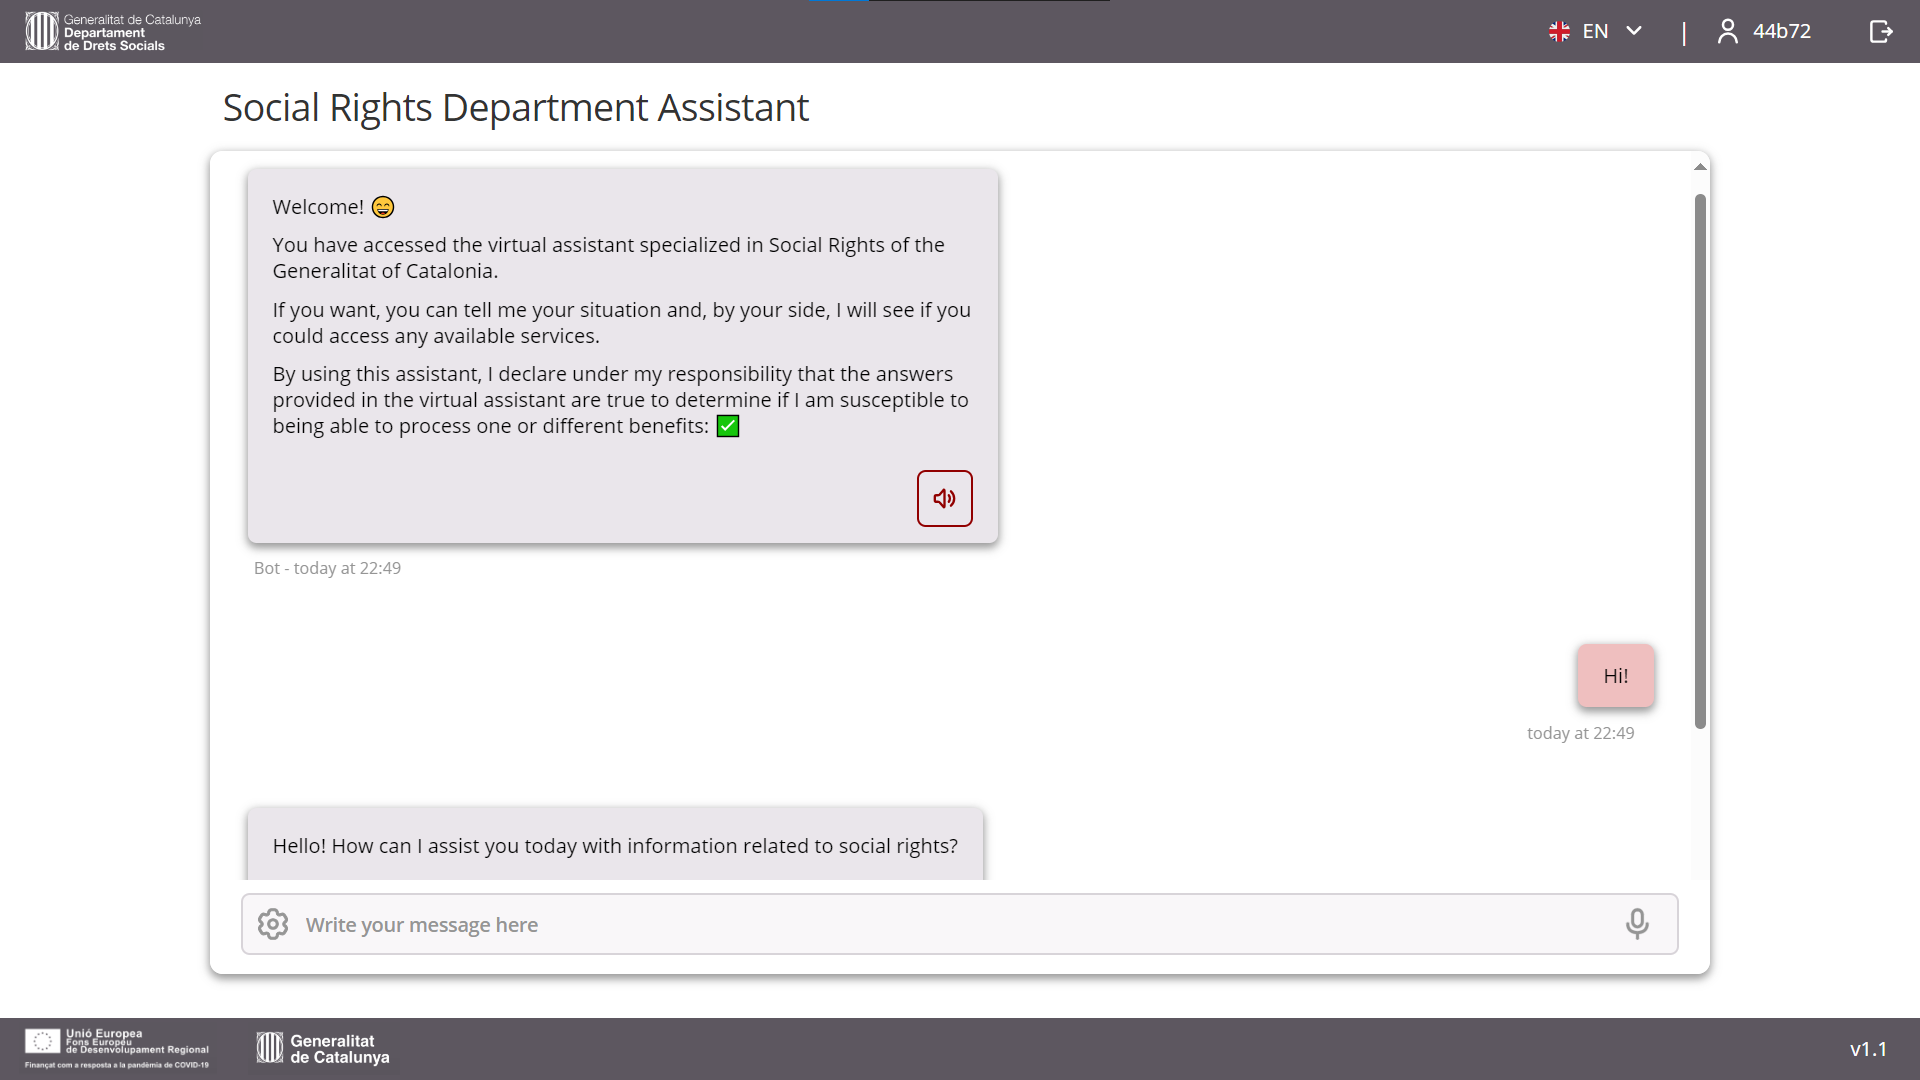
\includegraphics[width=1\textwidth]{img/UI Design.png}
  \caption{Frontend Interface}
  \label{fig:frontend}
\end{figure}

\subsection{Hotword/Wakeword Detection}
\label{subsec:hotword_detection}

On the frontend we implement a custom version of the EfficientWord-Net \cite{Chidhambararajan2022EfficientWordNet} hotword detector, that has been quantized \cite{Zhang2023PostTrainingQuantizationNeuralNetworks}. To implement it we use ONNX \cite{onnx} and WebAssembly (Wasm) \cite{wasm}, which run directly in the browser, ensuring no data leaves the client's machine inadvertently. The hotword detector listens to the microphone data in real-time, and when it hears the keyword ``chat'' or ``chatbot'', it activates the microphone and starts recording. We will see how this data is processed in the \ref{sec:azure_services} section.

The EfficientWord-Net model has been quantized to 8-bits, which has reduced the size of the model from 80MB to 20MB, and has improved the response time by 100\%. This has been achieved without perceptibly sacrificing the accuracy of the hotword detection.

The hotword detector analyzes audio data in chunks of 1.5 seconds, overlapped by 0.75 seconds. The raw audio signal is first converted to a Mel spectrogram (Figure~\ref{fig:mel_spectrogram}), which is then passed through a ResNet \cite{He2015DeepResidualLearningImage} model to generate semantic embedding vectors. These vectors are then compared to the embedding vectors of reference recordings of the hotword (which are prerecorded) using cosine similarity. If the similarity is above a certain threshold, the hotword is detected.
We use the pretrained model as provided by the EfficientWord-Net library, with no further training.

This approach works in a few-shot learning manner, as the model was never explicitly trained to recognize the specific hotword we use. Instead, it was trained to encode the semantic information of an audio signal using a large dataset of audio recordings and the reference recordings of the hotword are the few-shot examples that the model uses to learn to recognize the hotword. This approach is more efficient than training the model from scratch, as it leverages the model's pre-existing knowledge of audio signals to learn the new task, and it also allows us to deploy this model even though we are data-constrained (we have to record the references ourselves).

\begin{figure}[htb]
  \centering
  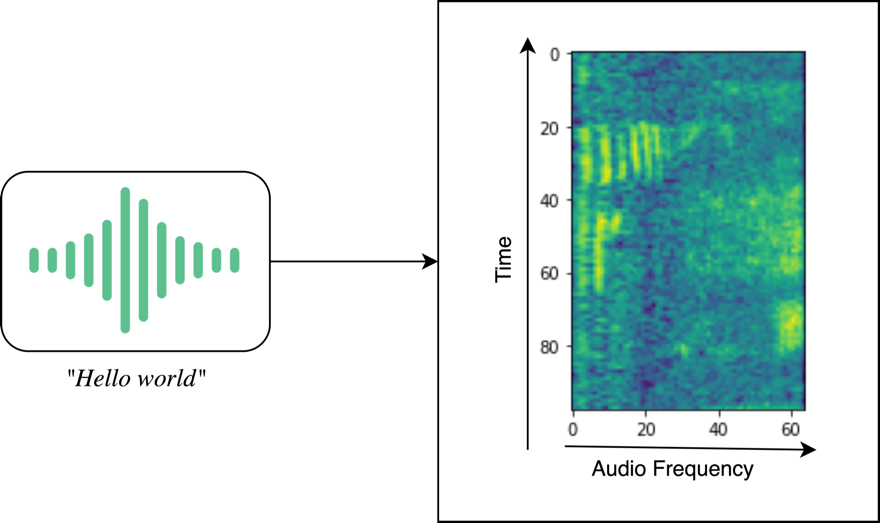
\includegraphics[width=1\textwidth]{img/MelSpectrogram.png}
  \caption{Mel spectrogram of the audio ``Hello world'' (image taken from \cite{Chidhambararajan2022EfficientWordNet})}
  \label{fig:mel_spectrogram}
\end{figure}

Because this system needs to run on the browser, and there is no existing implementation of a Mel spectrogram converter, we implement our own converter directly in TypeScript. This converter is as close as possible to a direct translation --from Python to TypeScript-- of the original code from the EfficientWord-Net library. By doing so we ensure data generated by our implementation is equivalent to that generated by the original implementation. We evaluate that this is the case by making bitwise comparisons of the output of both implementations (subtracting one image from the other), and find there are no differences (all pixels in the resulting image are exactly 0).

On our reference system, which consists of a Dell Latitude 3440 laptop with a 13th Gen Intel(R) Core(TM) i5-1345U CPU, the hotword detector has a response time of around 80-100 milliseconds, which is well within the acceptable range for real-time applications.

\section{Azure Services}
\label{sec:azure_services}

\subsection{Speech-to-Text}
\label{subsec:speech_to_text}

When the hotword detector activates the microphone, the audio data is sent to the Azure Speech-to-Text service. This service converts the audio data into text, which is then sent to the Backend for processing. The Azure Speech-to-Text service uses the Whisper \cite{Radford2022RobustSpeechRecognitionLargeScale} model to accurately transcribe speech into text.

\subsection{Text-to-Speech}
\label{subsec:text_to_speech}

From the frontend, a user can choose to have the chatbot's responses read out loud, by clicking on a button. When this happens, the text of the response is sent to the Azure Text-to-Speech service, which converts the text into audio data. This audio data is then sent back to the frontend, where it is played through the user's speakers.

\subsection{PostgreSQL Database}
\label{subsec:database}

The PostgreSQL database contains the text of the laws related to social rights and available social benefits in Catalonia. This data is indexed using the LlamaIndex Python library to chunk the text into smaller pieces, index them and  help create semantic embeddings. When a user query is received, the information retrieval system searches the database for the most relevant laws and benefits based on the query, and returns this information to the GPT model for generation.

\subsection{GPT Model}
\label{subsec:gpt_model}

The GPT model is used to generate coherent and contextually relevant responses to user queries based on the information retrieved from the database. The GPT model is a transformer-based \cite{Vaswani2023AttentionNeed} language model that is trained on a large dataset of text to generate human-like responses to user queries.

We use the GPT-4o and GPT-4o Mini models, which are the latest versions of the GPT model developed by OpenAI at the time of writing.

\section{Backend}
\label{sec:backend}

\subsection{Conversation Flow}
\label{subsec:conversation_flow}

The Backend implements, the conversation flow followed by the chatbot. It implements multiple stages and follows a state machine to manage the conversation. User queries at each stage are routed to the appropriate model.

Conversations flows are implemented using Flowable. Figures \ref{fig:conversation}, \ref{fig:antidan}, \ref{fig:treatscenario}, \ref{fig:answerragquestionifexists}, \ref{fig:executesituationdiscoveryscenario}, and \ref{fig:infervariablesprocess} show the flow diagrams for the different stages of the conversation.

At each stage the backend can decide to talk to one of the other components of the architecture. For example, during the RAG stage it uses our Vector Search API component to generate a response based on the information retrieved from the database. In another case, in the scenario where we are discovering the user's situation, the backend talks to the IA Social component to and asks it if, given the current conversation, there are any SNOMEDs that might apply to the user.

The backend also implements any error handling that might be necessary. The error handling is implemented directly on the flow diagram itself.

\section{Vector Search API}
\label{sec:vector_search_api}

As we needed to implement a few custom components all related to the RAG system, we decided to abstract them into a single separate component, the Vector Search API. This component is responsible for managing the information retrieval system, and for generating responses based on the information retrieved from the database. This component is abstract enough to be reused in chatbot systems other than the one we are developing for the DSO.

This API is implemented in Python using Flask to serve the API endpoints, and with Waitress as the WSGI server, as depicted in Figure \ref{fig:architecture}.

The following sections describe the features that this API provides.

\subsection{Model Routing}
\label{subsec:model_routing}

We use a slightly tweaked version of the fairly new RouteLLM Python library. This allows us to route a certain percentage of queries to a ``stronger'', more expensive model and the rest to a ``weaker'', less expensive model. With this system we are able to achieve X\% of the performance of the stronger model at a fraction of the cost. The RouteLLM system uses a small BERT classifier model that decides which queries should be routed to the stronger model and which to the weaker model. This classifier was trained by the original library authors on a dataset of human preferences augmented with synthetic data generated using GPT-4. They report good generalization performance, so we apply the system on a pair consisting of GPT-4o and GPT-4o Mini. We have also made the necessary changes to the library to make it compatible with the Azure OpenAI models, which didn't have official support.

We have translated the dataset the authors used to train the BERT classifier to Catalan, and are in the process of retraining the classifier on this new dataset, at the time of writing.

The translated training dataset consists of two parts: the translated texts and the embeddings of the texts. The translations were generated using the GPT-4o model and the embeddings using the \textit{text-embedding-3-large} model. The total cost of generating the translations and embeddings was around 500 euros. The datasets can be found here \href{https://huggingface.co/datasets/SupremeLobster/gpt4_judge_battles_catalan}{[translated texts]} and here \href{https://huggingface.co/datasets/SupremeLobster/gpt4_judge_battles_catalan_embeddings}{[embeddings]}.

\begin{figure}[H]
  \centering
  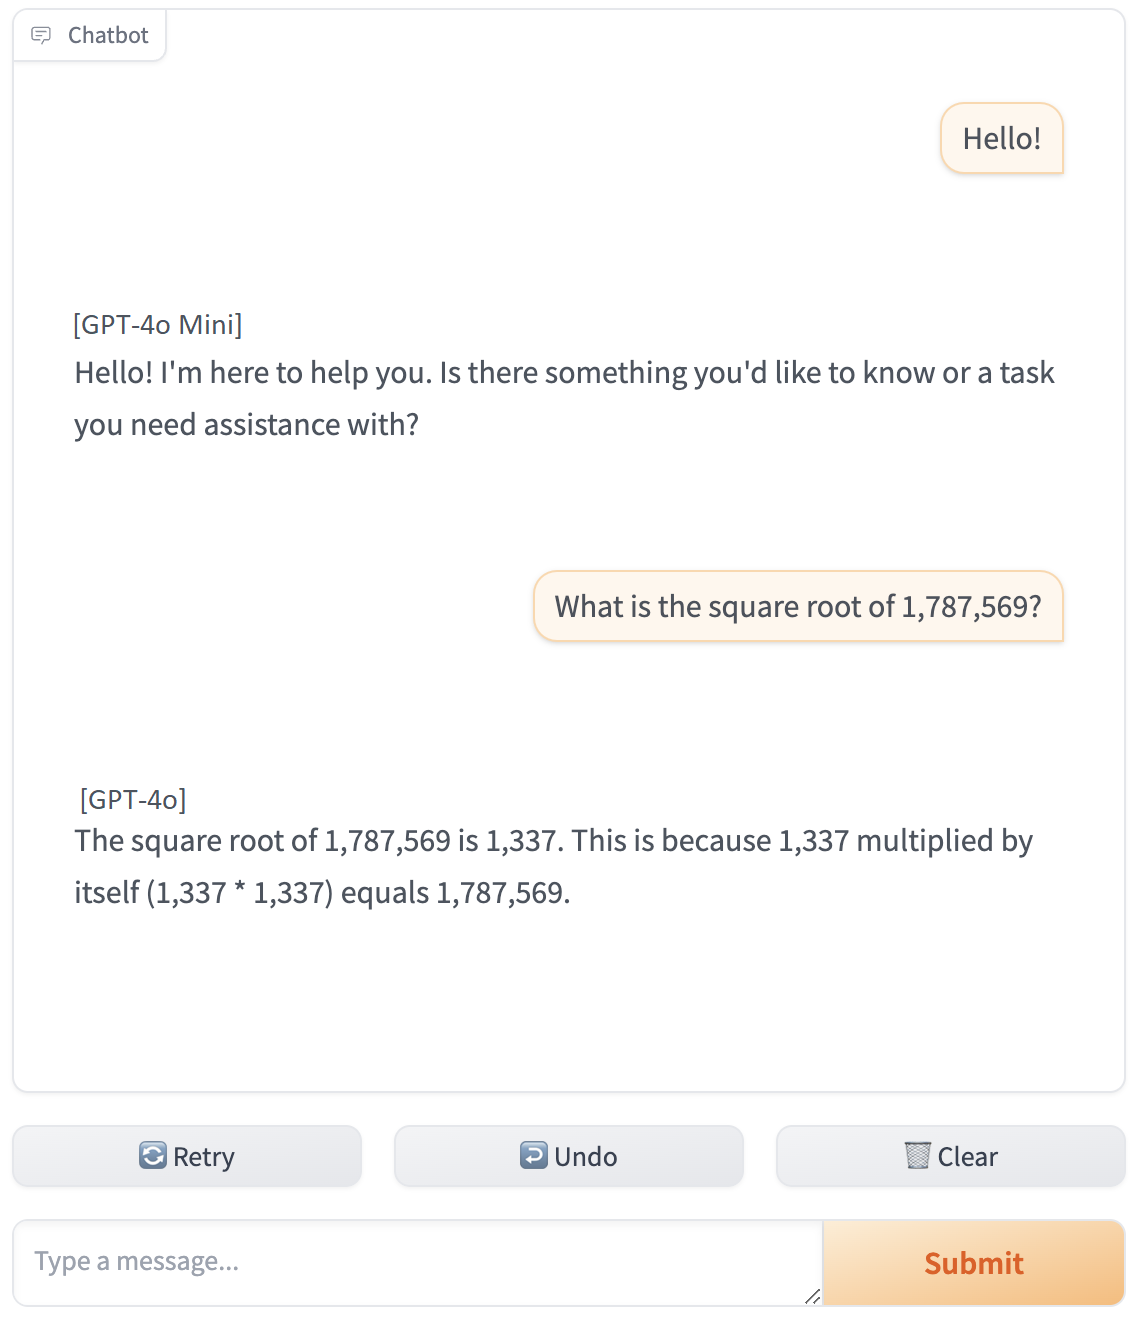
\includegraphics[width=0.5\textwidth]{img/Routed conversation.png}
  \caption{Example of conversation messages being routed to different models according to their complexity}
  \label{fig:model_routing_example}
\end{figure}

\subsection{Information Retrieval}
\label{subsec:information_retrieval}

We do RAG using the LlamaIndex python library.

We use two versions of RAG: normal RAG and Small To Big Retrieval (STBR).

\begin{itemize}
  \item \textbf{Normal RAG:} This is the standard RAG algorithm. It simply creates an embedding of the user query and does cosine similarity with the embeddings of the chunks in the database to retrieve the N most relevant chunks. In practice the database implements this with the Hierarchical Navigable Small World (HNSW) \cite{Malkov2018EfficientRobustApproximateNearestNeighbors} algorithm, which is a fast approximate nearest neighbor search algorithm, in order to avoid having to compare the user query with all the entries in the database's table. However this implementation is invisible, as the database itself executes it.
  \item \textbf{Small To Big Retrieval (STBR):} This is a less common RAG algorithm that uses hierarchical embeddings of chunks, allowing us to capture both fine-grained and coarse-grained information. Figure \ref{fig:SmallToBigRetrieval} shows our hierarchy-of-embeddings setup. Each level's embeddings correspond to smaller and smaller chunks of the text. We have 3 levels of embeddings. This can be thought of as analogous to the way a CNN model captures both fine-grained and coarse-grained information, where deeper layers have a larger receptive field. We implement the algorithm using the \href{https://docs.llamaindex.ai/en/stable/examples/retrievers/recursive_retriever_nodes/}{RecursiveRetriever class} from the LlamaIndex library.
  
  The STBR algorithm is implemented in the Vector Search API and runs at the top level, so the embedding searches are still performed by the database itself, still using the HNSW algorithm. Therefore STBR is more expensive because it performs multiple database queries (one per hierarchy level), but it is also more accurate for retrieving the most relevant information.
\end{itemize}

\begin{figure}[htb]
  \centering
  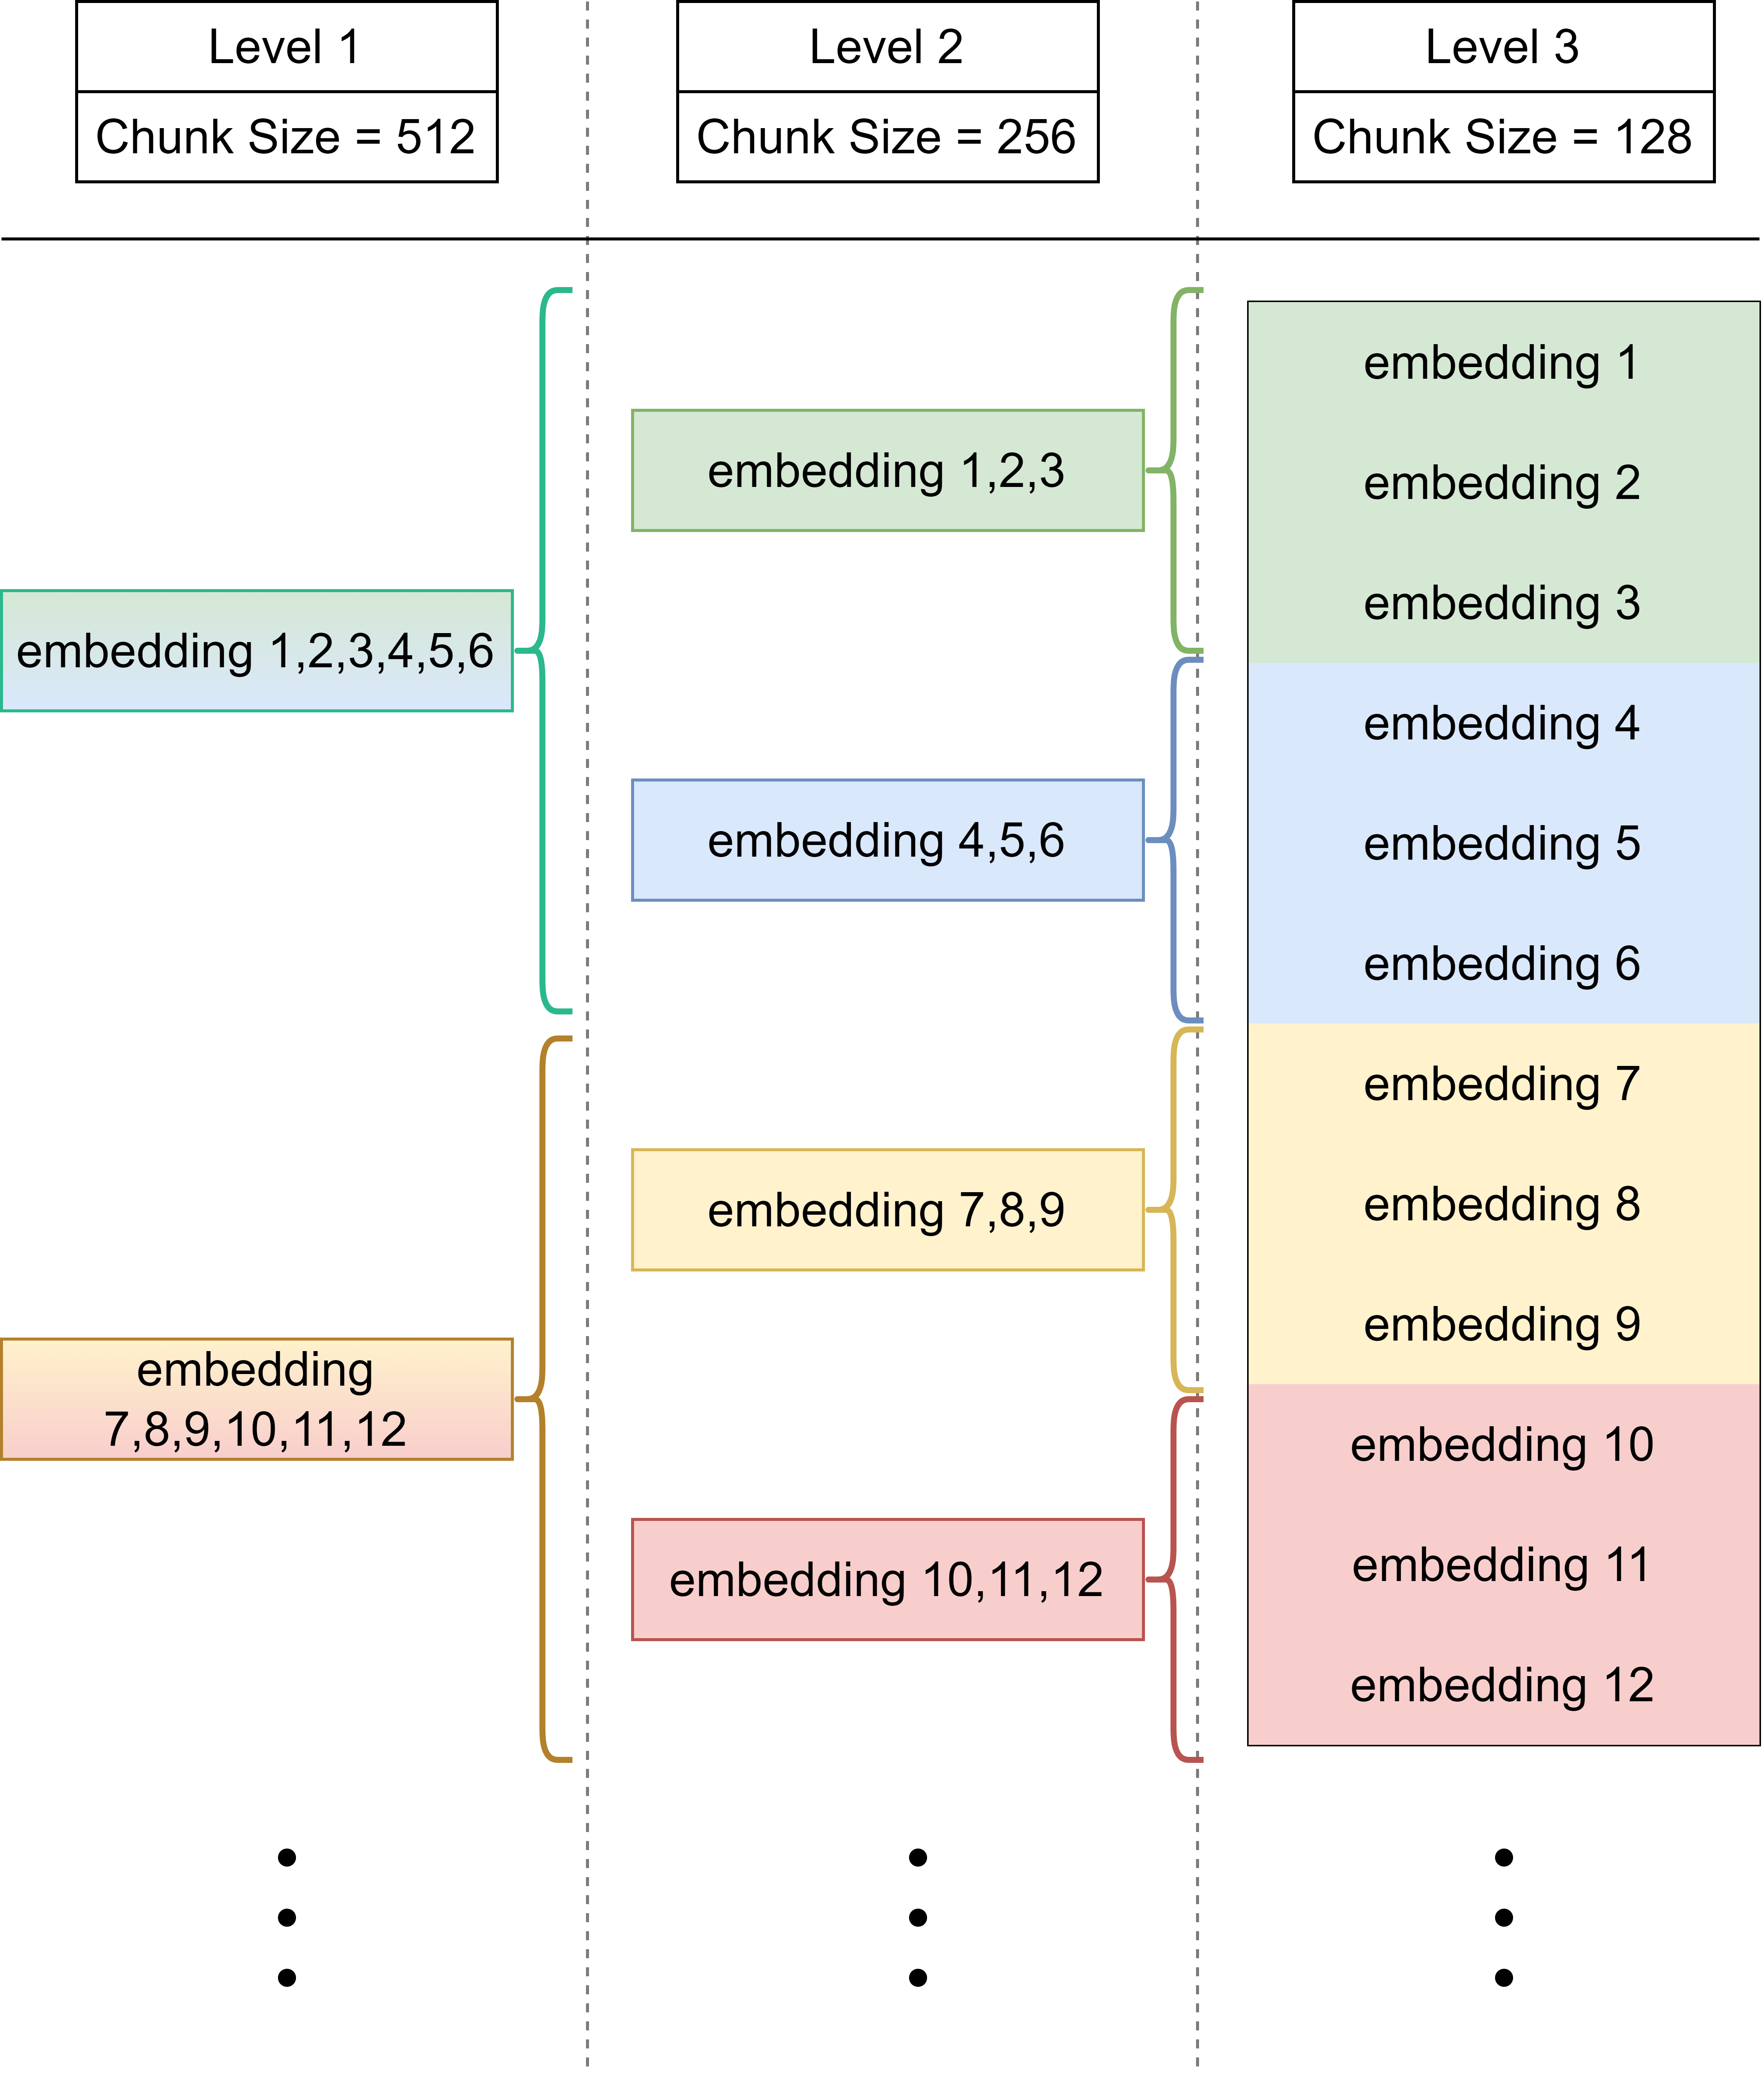
\includegraphics[width=0.5\textwidth]{img/Small To Big Retrieval.drawio.png}
  \caption{Small To Big Retrieval (STBR) embeddings hierarchy}
  \label{fig:SmallToBigRetrieval}
\end{figure}

\chapter{Results}
\label{cap:results}

Here we show the results of the performance of the RAG system in properly responding to user queries. We create a benchmark consisting of 35 questions to which we know the correct answers and evaluate the system's performance in answering them. We evaluate two systems: normal RAG and STBR. We evaluate the performance of the system in terms of accuracy. Both RAG systems will have access to the same database. We run the benchmark 4 times per system and average the results. We do this because the temperature of our system is greater than 0 (it's actually 0.1), so the responses are not deterministic. With this setup we are able to measure the robustness of the system.

Following the ideas of \cite{Es2023RagasAutomatedEvaluationRetrieval}, we use the GPT-4o model itself to evaluate it's performance by asking it to compare the generated answer to the correct answer and tell us if it is correct or not.

With the results produced, shown in Table \ref{tab:benchmark_results}, we can see that the STBR system outperforms the normal RAG system in terms of accuracy. The STBR system has an average accuracy of 0.79, while the normal RAG system has an average accuracy of 0.65. The standard deviation of the STBR system is also lower than that of the normal RAG system, indicating that the STBR system is more consistent in its performance. However the STBR is around 2x slower than normal RAG due to it performing a lot more database searches. Therefore we use the STBR system in cases where high accuracy is required, and the normal RAG system in cases where lower accuracy is acceptable but faster response times are needed.

\begin{table}[H]
  \centering
  \begin{tabular}{|c|c|c|}
    \hline
    \textbf{Question} & \textbf{Normal RAG Accuracy \(\uparrow\)} & \textbf{STBR RAG Accuracy \(\uparrow\)} \\
    \hline
    1                 & 0.0                          & 1.0                        \\
    2                 & 0.0                          & 0.0                        \\
    3                 & 1.0                          & 1.0                        \\
    4                 & 0.0                          & 1.0                        \\
    5                 & 1.0                          & 1.0                        \\
    6                 & 0.25                          & 1.0                        \\
    7                 & 1.0                          & 1.0                        \\
    8                 & 1.0                          & 1.0                        \\
    9                 & 0.25                          & 0.0                        \\
    10                & 0.25                          & 0.5                        \\
    11                & 1.0                          & 1.0                        \\
    12                & 1.0                          & 0.75                        \\
    13                & 1.0                          & 1.0                        \\
    14                & 1.0                          & 1.0                        \\
    15                & 1.0                          & 1.0                        \\
    16                & 0.75                          & 1.0                        \\
    17                & 1.0                          & 0.5                        \\
    18                & 1.0                          & 1.0                        \\
    19                & 0.75                          & 1.0                        \\
    20                & 1.0                          & 1.0                        \\
    21                & 0.0                          & 0.25                        \\
    22                & 0.0                          & 0.0                        \\
    23                & 1.0                          & 1.0                        \\
    24                & 1.0                          & 1.0                        \\
    25                & 0.0                          & 0.0                        \\
    26                & 1.0                          & 0.75                        \\
    27                & 1.0                          & 1.0                        \\
    28                & 0.0                          & 1.0                        \\
    29                & 0.0                          & 1.0                        \\
    30                & 1.0                          & 1.0                        \\
    31                & 1.0                          & 1.0                        \\
    32                & 1.0                          & 1.0                        \\
    33                & 0.5                          & 1.0                        \\
    34                & 0.0                          & 0.0                        \\
    35                & 1.0                          & 1.0                        \\
    \hline
    \textbf{Average \(\uparrow\)}  & 0.65                         & \textbf{0.79}                        \\
    \hline
    \textbf{STD \(\downarrow\)}      & 0.031                         & \textbf{0.024}                        \\
    \hline
  \end{tabular}
  \caption{Results of the benchmark. In bold we show the best result.}
  \label{tab:benchmark_results}
\end{table}

\section{Other Results}
\label{sec:other_results}

We were not able to conduct user testing as this product is not yet production ready as of the writing of this document. However, we have demoed the system to the stakeholders and they have expressed satisfaction with the results. They have also provided feedback on the system, which we will use to make improvements in future iterations. Mainly they have expressed the need for the system to be able to handle queries in a more natural way, which we already have plans to implement in the future.

\chapter{Conclusions}
\label{cap:conclusions}

In this project we have developed an advanced chatbot system that uses GPT technology and RAG to provide responses to user queries based on the content of a database. We have implemented a frontend interface that allows users to interact with the chatbot in a natural and intuitive way, and a backend system that manages the conversation flow and the calls to the language models and the database. We have also implemented a Vector Search API that manages the information retrieval system and generates responses based on the information retrieved from the database.

We have evaluated the performance of the RAG system in properly responding to user queries, and have found that the STBR system outperforms the normal RAG system in terms of accuracy. The STBR system has an average accuracy of 0.79, while the normal RAG system has an average accuracy of 0.65. The standard deviation of the STBR system is also lower than that of the normal RAG system, indicating that the STBR system is more consistent in its performance.

The chatbot system developed in this project has the potential to be a valuable tool for the Department of Social Rights of the Generalitat de Catalunya, providing users with accurate and relevant information on social rights and benefits in Catalonia. The system is designed to be flexible and adaptable, allowing for easy integration with other systems and databases. The use of RAG technology enhances the accuracy and relevance of the responses generated by the chatbot, improving the user experience and increasing the system's utility.

\section{Future Work}
\label{sec:future_work}

There are several areas for future work that could further enhance the capabilities and performance of the chatbot system developed in this project:

\begin{itemize}
  \item \textbf{Multilingual Support:} Implement support for additional languages to make the chatbot accessible to a wider range of users. This could involve training the language models on multilingual datasets and developing language-specific components for the information retrieval system.
  \item \textbf{Enhanced User Interface:} Improve the user interface to provide a more engaging and interactive experience for users. This could involve adding multimedia elements, such as images and videos, to the chat interface, and incorporating voice and gesture-based interactions.
  \item \textbf{Accessibility Features:} Implement additional accessibility features to make the chatbot more accessible to users with visual or motor impairments. This could include support for screen readers, voice commands, and other assistive technologies.
  \item \textbf{Performance Optimization:} Optimize the performance of the chatbot system to reduce response times and improve scalability. This could involve implementing caching mechanisms, load balancing, and other performance-enhancing techniques.
  \item \textbf{Continuous Improvement:} Conduct regular user testing and feedback sessions to identify areas for improvement and optimization. This could involve analyzing user feedback, monitoring system performance, and making iterative improvements to the chatbot system.
\end{itemize}

\section{Our Contributions to Open-Source}
\label{sec:oss_contributions}

During the development of this project we have iterated and made changes to a few existing tools and components. Here we link to our forks of the repositories.

\begin{itemize}
  \item EfficientWord-Net: \url{https://github.com/SupremeLobster/EfficientWord-Net} - Our fork of the EfficientWord-Net library, which has been modified to reduce response time, client machine requirements, and the size of downloaded files, through Quantization methods.
  
  We have opened a pull request with these changes to the original repository, which is still pending.
  \item RouteLLM: \url{https://github.com/SupremeLobster/RouteLLM} - Our fork of the RouteLLM library, which allows us to route a certain percentage of queries to a ``stronger'', more expensive model and the rest to a ``weaker'', less expensive model. Our changes are in the branch ``feature/support-azure-openai-embeddings''. These changes made the library compatible with the Azure OpenAI models, which didn't have official support.
  
  As of the time of writing, we are in the proces of cleaning up the code and opening a pull request with these changes to the original repository.
\end{itemize}

\backmatter

\bibliographystyle{ThesisStyleBreakable}
% \bibliographystyle{ieeetr}
\bibliography{biblio}

%\printnomenclature


\appendix
\include{Appendix1}

\chapter{Flowable Diagrams}
\label{cap:flowable_diagrams}

\begin{figure}[H]
  \centering
  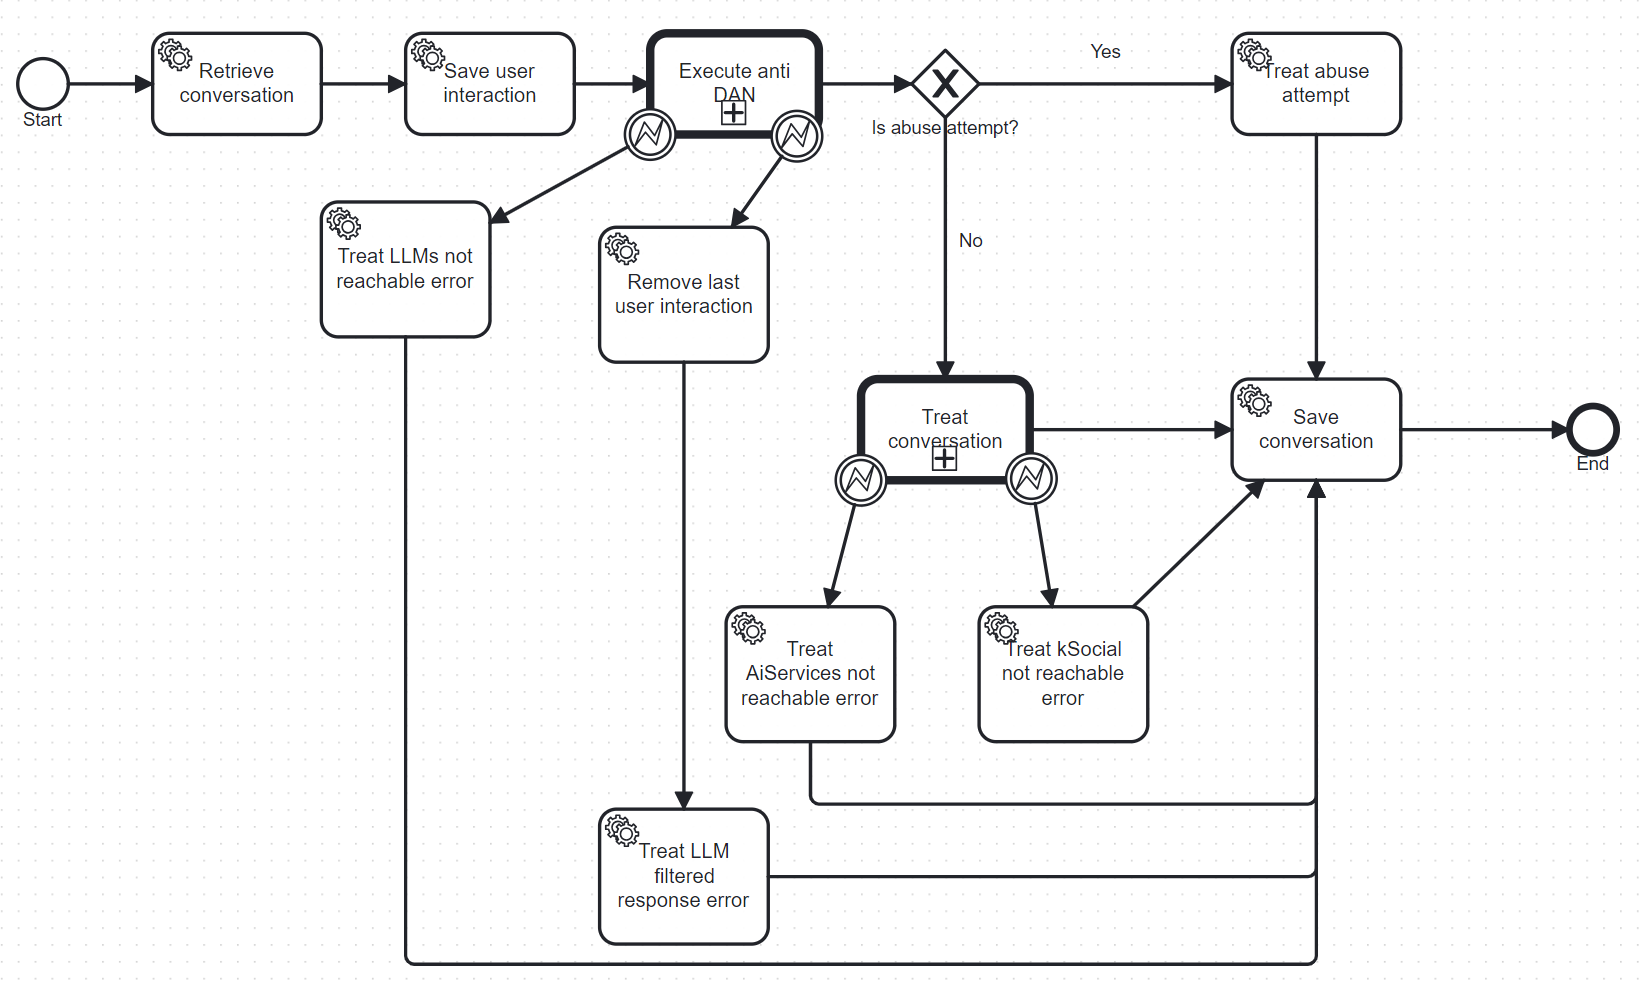
\includegraphics[width=1\textwidth]{img/Conversation_process.bpmn20.png}
  \caption{Top level flow diagram for the conversation}
  \label{fig:conversation}
\end{figure}

\begin{figure}[H]
  \centering
  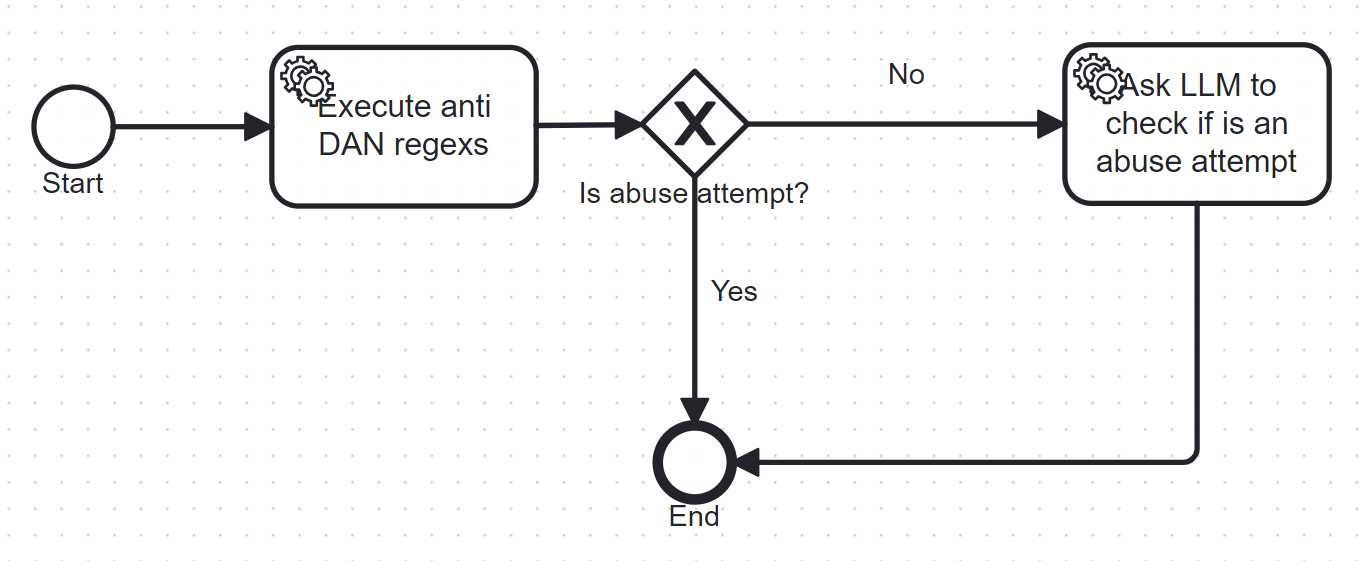
\includegraphics[width=1\textwidth]{img/Execute_anti_DAN.bpmn20.png}
  \caption{Flow diagram for the Anti DAN stage}
  \label{fig:antidan}
\end{figure}

\begin{figure}[H]
  \centering
  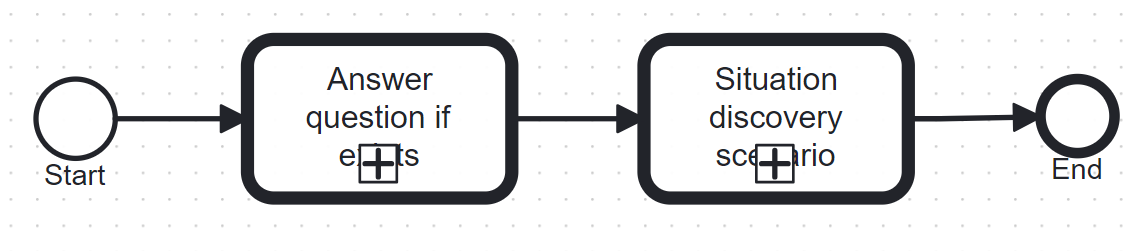
\includegraphics[width=1\textwidth]{img/Treat_conversation_scenario.bpmn20.png}
  \caption{Flow diagram for treating a scenario}
  \label{fig:treatscenario}
\end{figure}

\begin{figure}[H]
  \centering
  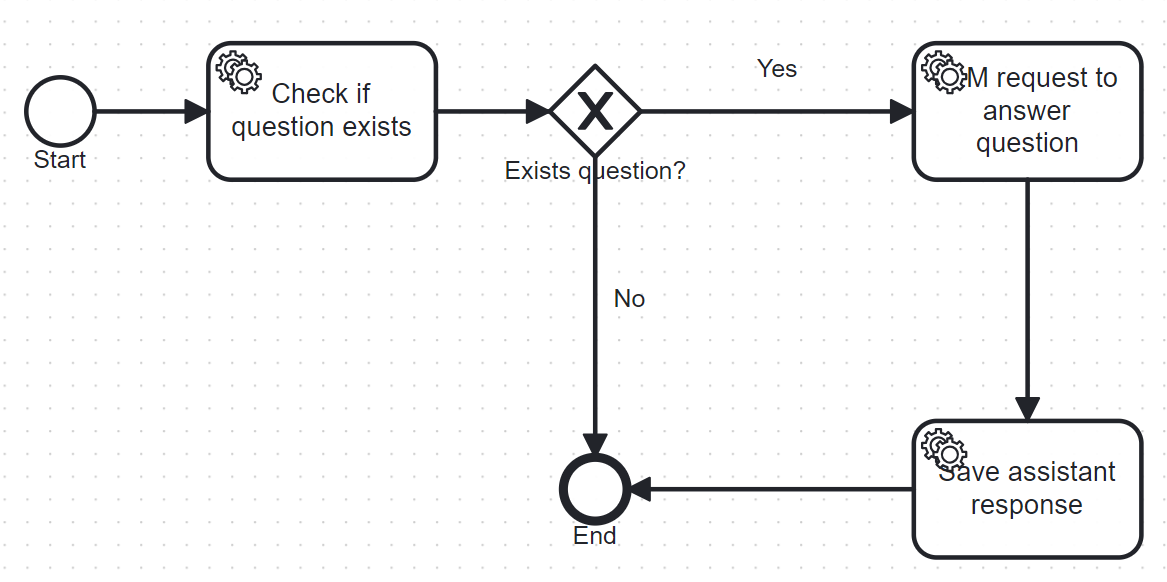
\includegraphics[width=1\textwidth]{img/Answer_question_if_exists.bpmn20.png}
  \caption{Flow diagram for the answering a question using RAG (if a question exists)}
  \label{fig:answerragquestionifexists}
\end{figure}

\begin{figure}[H]
  \centering
  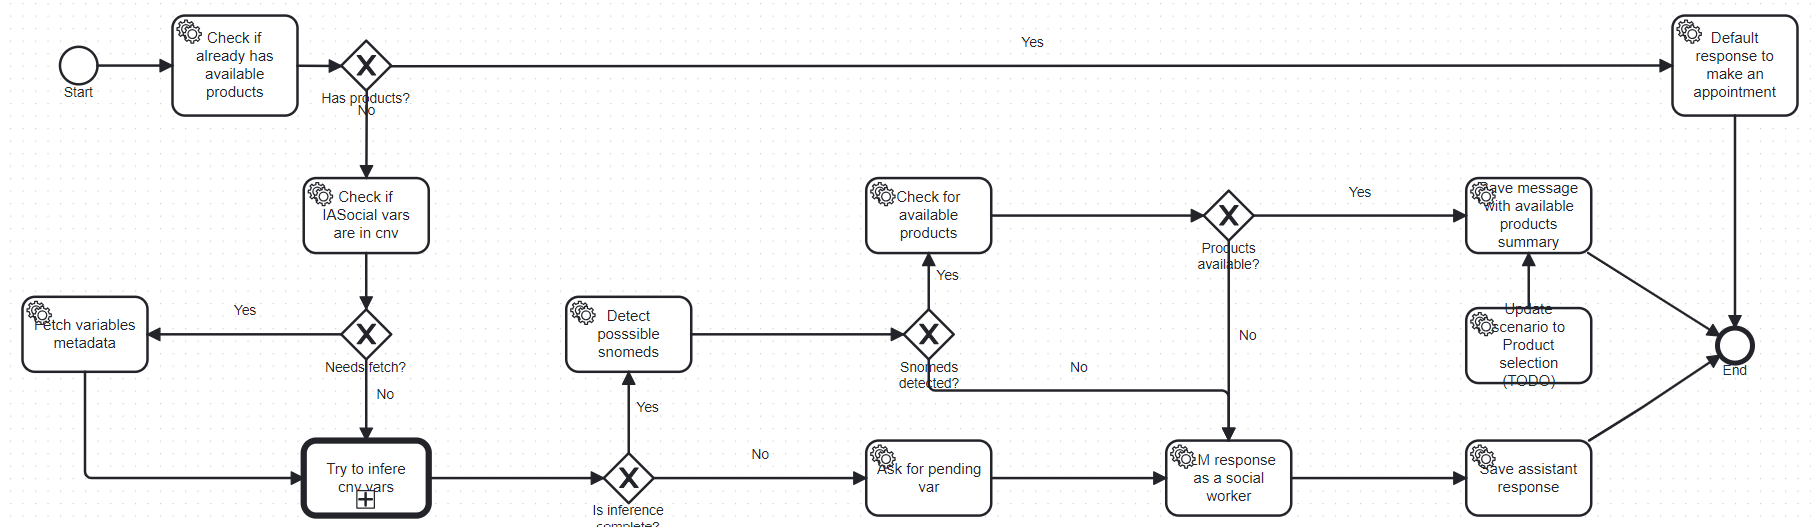
\includegraphics[width=1\textwidth]{img/Situation_discovery_scenario.bpmn20.png}
  \caption{Flow diagram for the scenario where we need to discover the user's situation}
  \label{fig:executesituationdiscoveryscenario}
\end{figure}

\begin{figure}[H]
  \centering
  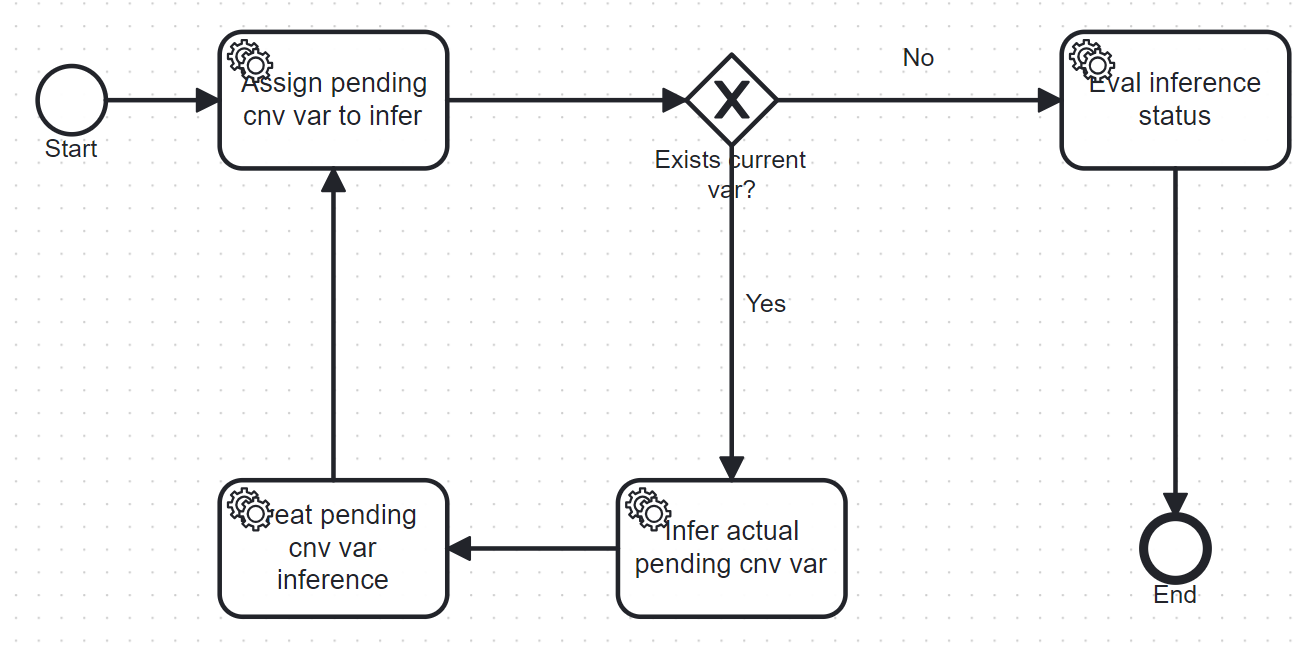
\includegraphics[width=1\textwidth]{img/Infere_conversation_variables.bpmn20.png}
  \caption{Flow diagram for inferring necessary variables for the current scenario based on the conversation}
  \label{fig:infervariablesprocess}
\end{figure}

\end{document}
